

%\renewcommand{\labelitemi}{\textbf{\alph{itemi}.)}}
%\renewcommand{\labelenumi}{\textbf{\arabic{enumi}.)}}
%\renewcommand{\labelenumii}{\textbf{\alph{enumi}.)}}

\section{Orthogonale Vektoren}
\subsection{Orthogonale Vektoren finden}
\begin{enumerate}
\item Die nächstliegendsten Vektorkombinationen sind:
  \begin{multicols}{4}
  \item[\textbf{a)}] 
    $ \Vektor{-1}{0}, \Vektor{1}{0}  $ 
  \item[\textbf{b)}]	
    $ \Vektor{-1}{1}, \Vektor{1}{-1} $	
  \item[\textbf{c)}] 
    $ \Vektor{-4}{3}, \Vektor{4}{-3}  $ 
  \item[\textbf{d)}] 
    $ \Vektor{-2}{-7}, \Vektor{2}{7}  $
  \end{multicols}
\item Man findet einen orthogonalen Vektor zu einem anderen, indem man 
  seine Koordinaten vertauscht und bei einer Koordinate das Vorzeichen
  wechselt. 
\item Der Punkt wird entlang einer Geraden verschoben.
\item Es gibt unendlich viele, da man die Gerade aus 3.) in einem
  dreidimensionalen Raum einfach im Kreis drehen könnte. Demnach sind
  es genauso viele Vektoren, wie ein Kreis Punkte
  hat. Veranschaulicht: Halte einen Stift in die Luft und bilde mit
  einem Finger eine dazu rechtwinklige Gerade. Dann drehe den
  Finger. Jegliche mögliche Position des Fingers bildet einen
  möglichen orthogonalen Vektor. 
  %% \begin{figure}[h] 
  %%   \centering
  %%   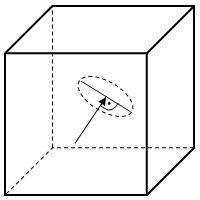
\includegraphics{pics/Vektor-Orthogonalitaet.jpg}
  %%   \caption{Unendlich viele Vektoren}
  %% \end{figure}
\item Es entsteht eine Ebene, die orthogonal zum ausgangsvektor
  liegt. Sind die Vektoren alle gleich lang, so enteht ein Kreis,
  dessen Mittelpunkt der nicht verschobene Punkt ist und dessen
  Radius gleich der Länge der Vektoren ist.
\item Man vertauscht zwei Koordinaten und ändert bei einer das
  Vorzeichen. Die dritte Koordinate wird auf 0 gesetzt.
  \begin{multicols}{4}
    \begin{enumerate}
    \item $  
      \begin{pmatrix}
        1\\0\\0
      \end{pmatrix}
      $
    \item $  
      \begin{pmatrix}
        1\\-1\\0
      \end{pmatrix}
      $
    \item $  
      \begin{pmatrix}
        -4\\0\\3
      \end{pmatrix}
      $
    \item $  
      \begin{pmatrix}
        1\\0\\-7
      \end{pmatrix}
      $
    \end{enumerate}
  \end{multicols}
\item Sie sind alle paarweise zueinander orthogonal, da sie alle eine
  jeweils andere Koordinate nicht 0 haben (sie sind jeweils parallel
  zu einer koordinatenachse).
\end{enumerate}
\subsection{Vektoren auf Orthogonalität prüfen}
	
	\begin{enumerate}
		\item
		\item[\textbf{Beispiel: d)}] 
		$ \Vektor{-7}{2}	\perp	\Vektor{-2}{-7}	\Leftrightarrow	(-7)\cdot(-2)+2\cdot(-7)	=+14-14	= 0 $ \\
		$ \Vektor{-7}{2}	\perp	\Vektor{2}{7}	\Leftrightarrow	(-7)\cdot2 + 2\cdot7		=-14+14	= 0 $
		
		\item
			\begin{multicols}{2}
				\item[\textbf{a.)}]
				$ 2\cdot(-6)+1\cdot12=0 \Leftrightarrow \Vektor{2}{1} \perp \Vektor{-6}{12}$\newline
				\item[\textbf{b.)}]
				$ 14\cdot4+(-8)\cdot7=0 \Leftrightarrow \Vektor{14}{4} \perp \Vektor{-8}{7}$\newline
				\item[\textbf{c.)}]
				$ (-1)\cdot4+(-4)\cdot1=-8 \Leftrightarrow \Vektor{2}{1} \not \perp \Vektor{-6}{12}$\newline
				\item[\textbf{d.)}]
				$ 7\cdot1+2\cdot(-3,5)=0 \Leftrightarrow \Vektor{7}{2} \perp \Vektor{1}{-3,5}$
			\end{multicols}
		

		\item
	Wir übernehmen den Satz des Pythagoras von oben: 
		$$|\vec{a}|^2 + |\vec{b}|^2 = |\vec{b} - \vec{a}|^2 $$
	und setzen die Vektoren ein:
		$$ \begin{array}{|c|}	\vektor{a_{1}}{a_{2}}{a_{3}} \end{array} ^2 + \begin{array}{|c|}\vektor{b_{1}}{b_{2}}{b_{3}} \end{array} ^2 = \begin{array}{|c|} \vektor{b_{1}}{b_{2}}{b_{3}} -	\vektor{a_{1}}{a_{2}}{a_{3}}\end{array} ^2  $$
	Wir beginnen mit den Rechenschritten um die Betragsstriche aufzulösen:
		$$ \sqrt{(a_1)^{2} + (a_{2})^2 + (a_{3})^2} ^2 + \sqrt{(b_1)^{2} + (b_{2})^2 + (b_{3})^2} ^2 = \sqrt{(b_1-a_1)^2 + (b_2-a_2)^2 + (b_3-a_3)^2}^2 $$
		Die $\sqrt{}$ können wir aufgrund des $^2$ einfach eliminieren und dann mithilfe der zweiten Binomischen Formel die Klammern rechts auflösen:
		$$ (a_1)^{2} + (a_2)^2 + (a_3)^2 + (b_1)^{2} + (b_2)^2 + (b_3)^2 = $$
		$$ (b_1)^2 - 2b_{1}a_{1} + (a_1)^2 + (b_2)^2 - 2b_{2}a_{2} + (a_2)^2 + (b_3)^2 - 2b_{3}a_{3} + (a_3)^2	$$
	Nun Streichen wir alles, was auf beiden Seiten vorkommt:
		$$ \cancel{(a_1)^{2}} + \cancel{(a_2)^2} + \cancel{(a_3)^2} + \cancel{(b_1)^2} + \cancel{(b_2)^2} + \cancel{(b_3)^2} =$$
		$$ \cancel{(b_1)^2} - 2b_{1}a_{1} + \cancel{(a_1)^2} + \cancel{(b_2)^2} - 2b_{2}a_{2} + \cancel{(a_2)^2} + \cancel{(b_3)^2} - 2b_{3}a_{3} + \cancel{(a_3)^2} $$
	Übrig bleibt:
		$$ 0 = 	- 2b_{1}a_{1} - 2b_{2}a_{2} - 2b_{3}a_{3} $$
	Wir teilen auf beiden Seiten der Gleichung durch -2 und erhalten: 
		$$ 0 = b_{1}a_{1} + b_{2}a_{2} + b_{3}a_{3} $$

		\item Wir benutzen unsere Erkenntnis aus \textbf{3.)} und setzen die Zahlen aus den Vektoren in die Gleichung ein. Wenn 0 heraus kommt, müssen die Vektoren orthogonal sein.
			\begin{multicols}{2}
				\item[\textbf{a.)}] 	$ 1\cdot0 + 1\cdot0 + 1\cdot0 = 0 $ 	\\ Also sind die Vektoren orthogonal.
				\item[\textbf{b.)}] 	$ 2\cdot(-4)+3\cdot0+4\cdot2=-8+8= 0$ 	\\ Also sind die Vektoren orthogonal.
				\item[\textbf{c.)}] 	$ 1\cdot2+2\cdot2+3\cdot(-2)=2+4-6=0$ 	\\ Also sind die Vektoren orthogonal.
				\item[\textbf{d.)}] 	$0\cdot0+0\cdot(-1)+2\cdot1=2$ 			\\ Also sind die Vektoren \underline{nicht} orthogonal.
			\end{multicols}
		
		
		\item
		Wir setzen jeweils in die Gleichung aus \textbf{3.)} ein und lösen nach a auf:
			\begin{multicols}{2}
				\item[\textbf{a.)}] $$ 3\cdot(-1) + 4\cdot2 + 1\cdot a = 0 $$
									$$ -3 + 8 + a = 0 	\qquad | +3 -8 $$ 
									$$ \uu{a = -5}$$
				\item[\textbf{b.)}] $$ 7\cdot1+1\cdot a+5\cdot2=0$$
									$$7+a+10=0 			\qquad |-17$$
									$$\uu{a=-17}$$
			\end{multicols}
			\begin{multicols}{2}	
				\item[\textbf{c.)}]	$$10\cdot a+27\cdot1+0,5\cdot(-14)=0$$
									$$10a+27-7=0 		\qquad |-20\quad |:10$$
									$$\uu{a=-2}$$
				\item[\textbf{d.)}] $$8\cdot2+3\cdot a+1\cdot a=0$$
									$$16+4a=0 			\qquad |-16 \quad |:4$$
									$$\uu{a=-4}$$
			\end{multicols}
	\end{enumerate}

\section{Skalarprodukt}
	\subsection{Skalarprodukt und Orthogonalität}	 
	\begin{enumerate}
 		\item \hfill
 			\begin{multicols}{2}
 				\item[\textbf{a.)}] $$ \Vektor{5}{0} 		\cdot \Vektor{1}{3} 	= 5\cdot1+0\cdot3=5  $$
 				\item[\textbf{b.)}]	$$ \vektor{1}{3}{1} 	\cdot \vektor{2}{5}{1} 	= 1\cdot2+3\cdot5+1\cdot1=18 $$
 				\item[\textbf{c.)}]	$$ \vektor{1}{3}{5}		\cdot \vektor{5}{3}{1} 	= 1\cdot5+3\cdot3+5\cdot1=19 $$
 				\item[\textbf{d.)}]	$$ \vektor{-11}{4}{1} 	\cdot \vektor{1}{2}{3} 	= (-11)\cdot1+4\cdot2+1\cdot3=0 $$
 			\end{multicols}
 		
 		\item Um zu überprüfen, ob die beiden Geraden orthogonal sind, genügt es uns, die Richtungsvektoren zu überprüfen. Wenn diese orthogonal zueinander liegen, tut das die ganze Gerade.
 		$$ \vektor{-5}{1}{0} \cdot \vektor{-2}{2}{0} = (-5)\cdot(-2)+1\cdot2+0\cdot0=10+2=12 \not = 0 \Leftrightarrow \vektor{-5}{1}{0} \not \perp \vektor{-2}{2}{0} $$ 		
 		
 		\item Hier denken wir uns einen unvollständigen Vektor aus, den wir als Richtungsvektor für die Gerade h nehmen. Der Einfachhalt halber hier: $\vektor{1}{1}{a}$.
 		Dann suchen wir a unter der Voraussetzung, dass der Vektor orthogonal zum Richtungsvektor von g ist.
 			\begin{multicols}{2}
	 			\item[\textbf{a.)}] $$ \vektor{7}{17}{-2} \perp \vektor{1}{1}{a} \Leftrightarrow  7\cdot1 + 17\cdot1 + (-2)\cdot a = 0 $$
 									$$7+17-2a=0 \qquad |-24 \quad |:(-2)$$
 									$$\uu{a=12}$$
 									$$\vektor{7}{17}{-2} \perp \vektor{1}{1}{12}$$
 				\item[\textbf{b.)}]	$$ \vektor{1}{2}{-3} \perp 				\vektor{1}{1}{a} \Leftrightarrow 1\cdot1 + 2\cdot1 + (-3)\cdot a = 0 $$
 									$$1+2-3a=0 \qquad |-3 \quad |:(-3)$$
 									$$\uu{a=1}$$
									$$\vektor{1}{2}{-3} \perp \vektor{1}{1}{1}$$
	 		\end{multicols}
 			
	 	\item Wir müssen jeweils Überprüfen, ob $\vec{AB}$, $\vec{BC}$ und $\vec{CA}$ orthogonal sind.
			\begin{multicols}{2}
				\item[\textbf{a.)}]	
							$\vec{AB}  = \vektor{3}{1}{4} $ 
				\item[]		$\vec{BC}  = \vektor{-1}{-3}{-5} $  	
				\item[]		$\vec{CA}  = \vektor{-2}{2}{1} $
 				\item[] 	$\vec{AB} \cdot \vec{BC} = \vektor{3}{1}{4} 	\cdot \vektor{-1}{-3}{-5} 	= -3-3-20 \not= 0 $ 
 				\item[]		$\vec{BC} \cdot \vec{CA} = \vektor{-1}{-3}{-5} 	\cdot \vektor{-2}{2}{1} 	= 2-6-5 \not= 0 $
 				\item[] 	$\vec{CA} \cdot \vec{AB} = \vektor{-2}{2}{1} 	\cdot \vektor{3}{1}{4} 		= -6 +2 +4 = 0$ 
 				\item[]
				\item[$\Leftrightarrow$]	
   							$\vec{CA} \perp \vec{AB} $
 			\end{multicols}		
 		
\bigskip	
			\begin{multicols}{2}
				\item[\textbf{b.)}]	
						$\vec{AB}  = \vektor{1}{-3}{-1} $ 
				\item[]	$\vec{BC}  = \vektor{-5}{-3}{4} $ 
				\item[]	$\vec{AB} \cdot \vec{BC} = \vektor{1}{-3}{-1} 	\cdot \vektor{-5}{-3}{4} 	=$ \\ $ 1\cdot(-5) + (-3)\cdot(-3) + (-1)\cdot4 = $\\$-5+9-4 = 0 $ 
	 			\item[$\Leftrightarrow$] $\vec{CA} \perp \vec{AB}$
 			\end{multicols}
	\item
%Wir suchen einen Vektor, für den die Gleichung aus 3.) für beide Vektoren gilt: \\
%			$$\vektor{1}{2}{3} \cdot \vektor{x}{y}{z} =0 \hspace{3cm} \vektor{2}{0}{3} \cdot \vektor{x}{y}{z} =0  $$
%		Wir rechnen das Skalarprodukt aus und erhalten zwei Gleichungen eines Gleichungssystems:
%			$$ \begin{array}{rrrr}
% 			1x&+2y&+3z &= 0 \\
%			2x&&+3z&=0 
%			\end{array}$$
%		Da wir drei Unbekannte aber nur zwei Gleichungen haben, können wir 	

		\item Wir müssen alles Winkel auf Orthogonalität überprüfen oder bis wir ein Gegenbeweis gefunden haben.
			\setlength{\columnsep}{-5cm}
			\begin{multicols}{2}
				\item[\textbf{a.)}]	
						$\vec{AB}  = \vektor{-1}{-2}{-1} $ 
				\item[]	$\vec{BC}  = \vektor{-11}{1}{9} $  	
				\item[]	$\vec{CD}  = \vektor{1}{2}{1} $
				\item[] $\vec{DA}  = \vektor{11}{-1}{-9} $
				\item[] $\vec{AB} \cdot \vec{BC} = \vektor{-1}{-2}{-1} 	\cdot \vektor{-11}{1}{9} 	= 11-2-9 = 0 $ 
				\item[]	$\vec{BC} \cdot \vec{CD} = \vektor{-11}{1}{9} 	\cdot \vektor{1}{2}{1} 		= -11+2+9 = 0 $
				\item[]	$\vec{CD} \cdot \vec{DA} = \vektor{1}{2}{1} 	\cdot \vektor{11}{-1}{-9} 	= 11-1-9 = 0 $
				\item[] $\vec{DA} \cdot \vec{AB} = \vektor{11}{-1}{-9} 	\cdot \vektor{-1}{-2}{-1} 	= -11+2+9 = 0$ 
 			\end{multicols}
\medskip
 			\setlength{\columnsep}{-5cm}
 			\begin{multicols}{2}
 				\item[\textbf{b.)}]	
 						$\vec{AB}  = \vektor{-1}{-1}{7} $ 
 				\item[]	$\vec{BC}  = \vektor{-5}{8}{-1} $  	
 				\item[] $\vec{AB} \cdot \vec{BC} = \vektor{-1}{-1}{7} 	\cdot \vektor{-5}{8}{-1} 	= 5-8-7 \not= 0 $ 
 				\item[]	$\Leftrightarrow \vec{AB} \not\perp \vec{BC}$
 			\end{multicols}
\medskip
 			\setlength{\columnsep}{-5cm}
 			\begin{multicols}{2}
 				\item[\textbf{7.)}]	$\vec{AC}  = \Vektor{5}{5} $ 
 				\item[]	$\vec{BD}  = \Vektor{3}{-3} $  	
 				\item[] $\vec{AC} \cdot \vec{BD} = \Vektor{5}{5} 	\cdot \Vektor{3}{-3} 	= 15-15 = 0 $ 
 				\item[]	$\Leftrightarrow \vec{AC} \perp \vec{BD}$
 			\end{multicols}
 	\end{enumerate}
\subsection{Winkelberechnung mithilfe des Skalarprodukts}
	\begin{enumerate}
		\item Da $\cos(90^\circ)=0$ kommt bei einem rechten Winkel mit der Gleichung $\vec{a}\cdot\vec{b}=|\vec{a}|\cdot|\vec{b}|\cdot0 $ stets Null raus. Demnach ist $\vec{a}\cdot\vec{b} = 0$ stets ein Zeichen für Orthogonalität.

		\item * Wir beginnen mit dem Kosinussatz, geben ihm Vektoren-Einheiten und formen um:
		
		{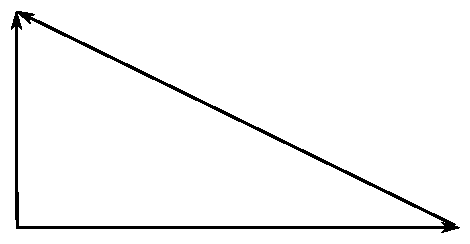
\includegraphics [keepaspectratio,height=5cm]{pics/Dreieck.jpg}}
		$$a=\vec{AB}=\vektor{a_1}{a_2}{a_3}$$			$$b=\vec{BC}=\vektor{b_1}{b_2}{b_3}$$
		$$c=\vec{CA}=\vektor{c_1}{c_2}{c_3}$$\newline\newline
Wir nehmen den Kosinussatz:				
		$$ a^2=b^2+c^2-2ab\cdot cos(\alpha)$$
Dort setzten wir die Bezeichnungen in Vektoren-Schreibweise hinein:	
		$$ |\vec{BC}|^2=|\vec{CA}^2|+|\vec{AB}|^2-2|\vec{CA}||\vec{AB}|\cdot cos(\alpha) $$
Wir tauschen $\vec{BC}$ mit $\vec{CA-AB}$ um nur noch zwei statt drei unterschiedlicher Vektoren zu haben:	
		$$|\vec{CA}-\vec{AB}|^2=|\vec{CA}|^2+|\vec{AB}|^2-2|\vec{CA}||\vec{AB}|\cdot cos(\alpha) \qquad |-|\vec{CA}|^2-|\vec{AB}|^2 $$
Dann fangen wir die Formel nach $\alpha$ umzustellen:	
		$$|\vec{CA}-\vec{AB}|^2-|\vec{CA}|^2-|\vec{AB}|^2=-2|\vec{CA}||\vec{AB}|\cdot \cos(\alpha) $$
Wir schreiben die Vektoren ganz auf,	
		$$\left|\vektor{c_1-a_1}{c_2-a_2}{c_3-a_3}\right|^2-\left|\vektor{c_1}{c_2}{c_3}\right|^2-\left|\vektor{a_1}{a_2}{a_3}\right|^2=-2|\vec{CA}||\vec{AB}| \cdot \cos(\alpha) $$
Um sie dann besser auseinanderziehen zu können:	
		$$\sqrt{(c_1-a_1)^2+(c_2-a_2)^2+(c_3-a_3)^2}^2-\sqrt{{c_1}^2+{c_2}^2+{c_3}^2}^2-\sqrt{{a_1}^2+{a_2}^2+{a_3}^2}^2=$$
		$$-2|\vec{CA}||\vec{AB}|\cdot \cos(\alpha) $$
Die Wurzeln und die Quadrate eliminieren sich:	
		$$(c_1-a_1)^2+(c_2-a_2)^2+(c_3-a_3)^2-{c_1}^2+{c_2}^2+{c_3}^2-{a_1}^2+{a_2}^2+{a_3}^2=$$
		$$-2|\vec{CA}||\vec{AB}|\cdot \cos(\alpha) $$
Und nach dem Anwenden der 2. Binomischen Formel eliminiert sich einiges in der Formel selbst:		
		$$\cancel{{c_1}^2}-2c_1a_1+\cancel{{a_1}^2}\quad+\quad\cancel{{c_2}^2}+-c_2+a_2+\cancel{{a_2}^2}\quad+\quad\cancel{{c_3}^2}-2c_3+a_3+\cancel{{a_3}^2}\quad-\cancel{{c_1}^2}+\cancel{{c_2}^2}+\cancel{{c_3}^2}-\cancel{{a_1}^2}+\cancel{{a_2}^2}+\cancel{{a_3}^2}=$$
		$$-2|\vec{CA}||\vec{AB}|\cdot \cos(\alpha) $$
Jetzt ziehen wir noch den Rest der rechten Seite auf die Linke, um $\cos(\alpha)$ alleine zu haben:
		$$-2c_1a_1-2c_2a_2-2c_3a_3=-2|\vec{CA}||\vec{AB}|\cdot \cos(\alpha) \qquad | :-2|\vec{CA}||\vec{AB}|$$
Als letztes Kürzen wir mit $-2$ und können aus dem Rest oberhalb des Bruches wieder zwei Vektoren bilden ($\vec{a}\cdot\vec{c}=a_1c_1+a_2c_2+a_3c_3$):	
		$$\dfrac{\cancel{-2}c_1a_1+\cancel{-2}c_2a_2+\cancel{-2}c_3a_3}{\cancel{-2}|\vec{CA}||\vec{AB}|}=\dfrac{c_1a_1+c_2a_2+c_3a_3}{|\vec{CA}||\vec{AB}|}=\dfrac{\vec{CA}\cdot\vec{AB}}{|\vec{CA}||\vec{AB}|}=\cos(\alpha)$$
	

	
		\item
			\begin{enumerate}
				\item[\textbf{a.)}]	$$ \cos(\alpha)=\dfrac{\Vektor{5}{0} \cdot \Vektor{1}{3}} {\left|\Vektor{5}{0}\right| \cdot \left| \Vektor{1}{3}\right|}=\dfrac{5\cdot1+3\cdot0} {\sqrt{5^2} \cdot \sqrt{3^2+1^2}} $$
								
				$$ \cos(\alpha)=\dfrac{\cancel{5}}{\cancel{5}\cdot\sqrt{10}} \qquad \left|\cos{}^{-1}\right.$$ 
								
				$$\alpha=\cos^{-1}\left(\dfrac{1}{\sqrt{10}}\right)$$
				
				$$\uu{\alpha = 71\mathrm{,}57^\circ}$$
\medskip
				\item[\textbf{b.)}]			
				$$\alpha=\cos^{-1}\left(\cfrac{2+15+1}{\sqrt{1+9+1}\cdot\sqrt{4+25+1}}\right)=\cos^{-1}\left(\cfrac{18}{\sqrt{11}\cdot\sqrt{30}}\right)=7\mathrm{,}75^\circ$$
				\item[\textbf{c.)}]	$$\alpha=\cos^{-1}\left(\cfrac{5+9+5}{\sqrt{1+9+25}\cdot\sqrt{25+9+1}}\right)=\cos^{-1}\left(\cfrac{19}{\sqrt{35}\cdot\sqrt{35}}\right)=57\mathrm{,}12^\circ$$
				\item[\textbf{d.)}]	$$\alpha=\cos^{-1}\left(\cfrac{-11+8+3}{\sqrt{144+16+1}\cdot\sqrt{1+4+9}}\right)=\cos^{-1}\left(\cfrac{0}{\sqrt{161}\cdot\sqrt{14}}\right)=90^\circ$$	
		\end{enumerate}
		\hfill\newline
		\end{enumerate}
%Neuaufsetzung wegen komischen Einschubs		
		\begin{enumerate}
		\setcounter{enumi}{3}
			\item 
				\begin{enumerate}
					\setcounter{enumii}{1}
				\item	$\vec{AB}=\Vektor{3}{-2} \qquad \vec{BC}=\Vektor{-1}{4} \qquad \vec{CA}=\Vektor{-2}{-2}$
\bigskip\newline
				$  a=|\vec{BC}| = \left|\Vektor{-1}{4}\right| = \sqrt{(-1)^2+4^2} = \sqrt{1+16} = \sqrt{17}\\ b=|\vec{CA}|=\left|\Vektor{-2}{-2}\right| = \sqrt{(-2)^2+(-2)^2} = \sqrt{4+4}=\sqrt{8}\\ c=|\vec{AB}| = \left|\Vektor{3}{-2}\right| = \sqrt{3^2+(-2)^2} = \sqrt{9+4} =\sqrt{13}$\\
\bigskip\newline
				$ \alpha = cos^{-1} \left(\frac{\vec{AB} \cdot \vec{CA}}{|\vec{AB}|\cdot |CA|}\right) = cos^{-1} \left(\frac{-6+4}{\sqrt{13} \cdot \sqrt{8}}\right) = 78\mathrm{,} 69^\circ $\\
					$ \beta = cos^{-1} \left(\frac{\vec{AB}\cdot\vec{BC}}{|\vec{AB}|\cdot|BC|}\right)=cos^{-1} \left(\frac{-3-8}{\sqrt{13}\cdot\sqrt{17}}\right) =42,27^\circ$\\
				$ \gamma = cos^{-1} \left(\frac{\vec{BC}\cdot\vec{CA}}{|\vec{BC}|\cdot|CA|}\right)=cos^{-1} \left(\frac{2-8}{\sqrt{17}\cdot\sqrt{8}}\right) =102,96^\circ $
			\end{enumerate}
			
			\bigskip
			\item 	
					\begin{enumerate}									
				\item	$\cos(30) =\dfrac{\vektor{0}{1}{0} \cdot \vektor{\sqrt{3}}{b}{0}} {\left|\vektor{0}{1}{0}\right| \cdot \left|\vektor{\sqrt{3}}{b}{0}\right|} = \dfrac{b}{\sqrt{3+b^2}}      \qquad \left|\cdot \sqrt{3+b^2}\right.$\\
						
						$\cos(30) \cdot \sqrt{3+b^2} = b 							\umf{^2}$ \\
						 
						$\cos(30)^2 \cdot (3+b^2) = b^2$\\
						 
						$\cos(30)^2 \cdot 3 + \cos(30)^2 \cdot b^2 = b^2      \qquad \left|-b^2\cdot cos(30)^2\right.$\\
						 
						$\cos(30)^2 \cdot 3 = 1 \cdot b^2 - (\cos(30)^2 \cdot b^2) $\\
						 
						$\cos(30)^2 \cdot 3 = b^2 \cdot (1-cos(30)^2) \umf{:(1-cos(30))}$\\
						 
						$\dfrac{\cos(30)^2 \cdot 3}{1-cos(30)^2}=b^2 \umf{\sqrt{~}}$\\
						
						$\dfrac{\sqrt{\cos(30)^2 \cdot 3}}{\sqrt{1-cos(30)^2}}=b$\\
						
						$\uu{\pm3=b}$
						 
			\item		
			\end{enumerate}			
			
					
		\end{enumerate}

